\section{addDipendente(DipendenteRequest request, String aliasAgenzia)}

Il metodo \textit{addDipendente}, appartenente alla classe UserService, ha la responsabilità di aggiungere al sistema un nuovo dipendente, che può essere un agente o un manager.

Per questo metodo è stata adottata una strategia di\textbf{ Black Box} Testing, poiché l’obiettivo principale è verificare il comportamento del sistema in base agli stati e ai valori dei parametri in ingresso, senza considerare la logica interna dell’implementazione. In particolare, si è ritenuto fondamentale analizzare le diverse condizioni in cui un dipendente viene correttamente registrato o rifiutato dal sistema.

A tal fine, è stata effettuata una suddivisione dei parametri di input in \textbf{classi di equivalenza}, al fine di individuare i casi validi e non validi da sottoporre a test. Di seguito si riportano le tabelle che documentano tale suddivisione:

\begin{table}[H]
	\centering
	\begin{tabular}{|c|p{4cm}|p{5cm}|c|} 
		\hline
		\textbf{ID Classe} & \textbf{Descrizione} & \textbf{Valore esempio} & \textbf{Validità} \\
		\hline
		DRN1 & L'insieme delle stringe non vuote/lunghezza zero
		& request.nome==Roberto; & Valido \\
		\hline
		DRN2 & L'insieme delle stringhe null/lunghezza zero
		& request.nome=="" & Non Valido \\
		\hline
	\end{tabular}
	\caption{Parametro DipendenteRequest.nome}
	\label{tab:parametriDipendenteRequestNome}
\end{table}

\begin{table}[H]
	\centering
	\begin{tabular}{|c|p{6cm}|p{5cm}|c|} 
		\hline
		\textbf{ID Classe} & \textbf{Descrizione} & \textbf{Valore esempio} & \textbf{Validità} \\
		\hline
		DRC1 & L'insieme delle stringe non vuote/lunghezza zero
		& request.cognome==Morosini; & Valido \\
		\hline
		DRC2 & L'insieme delle stringhe null/lunghezza zero
		& request.cognome==null & Non Valido \\
		\hline
	\end{tabular}
	\caption{Parametro DipendenteRequest.cognome}
	\label{tab:parametriDipendenteRequestCognome}
\end{table}

\begin{table}[H]
	\centering
	\begin{tabular}{|c|p{4cm}|p{5.5cm}|c|} 
		\hline
		\textbf{ID Classe} & \textbf{Descrizione} & \textbf{Valore esempio} & \textbf{Validità} \\
		\hline
		DRR1 & Stringa di valore "AGENT"
		& request.ruolo=="AGENT"; & Valido \\
		\hline
		DRR2 & Stringa di valore "MANAGER"
		& request.ruolo=="MANAGER" & Valido \\
		\hline
		DRR3 & tutti i valori non corrispodenti ad AGENT oppure a MANAGER
		& request.ruolo=="ADMIN" & Non Valido \\
		\hline
		DRR4 & stringa null/lunghezza zero
		& request.ruolo=="" & Non Valido \\
		\hline
	\end{tabular}
	\caption{Parametro DipendenteRequest.ruolo}
	\label{tab:parametriDipendenteRequestRuolo}
\end{table}

\begin{table}[H]
	\centering
	\begin{tabular}{|c|p{4cm}|p{5.5cm}|c|} 
		\hline
		\textbf{ID Classe} & \textbf{Descrizione} & \textbf{Valore esempio} & \textbf{Validità} \\
		\hline
		AA1 & L'insieme delle stringhe non null e non vuoti & aliasAgenzia==RobyImmobili & Valida \\
		\hline
		AA2 & La stringa è null oppure è vuota & aliasAgenzia==null & Non valido \\
		\hline
	\end{tabular}
	\caption{Parametro aliasAgenzia}
	\label{tab:parametriAliasAgenzia}
\end{table}

\vspace{1cm}

Per quanto riguarda la strategia di combinazione dei valori, è stato scelto l’approccio \textbf{R-WECT (Reduced Weak Equivalence Class Testing)}. Questa tecnica è considerata particolarmente robusta perché garantisce:

\begin{itemize}
	\item il test di tutte le classi non valide, ognuna combinata con valori validi per gli altri parametri;
	\item il test di tutte le classi valide per ciascun parametro.
\end{itemize}

Infine, vengono riportati sia il codice sorgente dei test implementati sia l’evidenza del loro esito positivo, a conferma della correttezza delle funzionalità verificate

% Definizione dei colori
\definecolor{bgcolor}{RGB}{245,245,245}    % Sfondo chiaro
\definecolor{keywordcolor}{RGB}{0,0,180}  % Blu per le parole chiave
\definecolor{commentcolor}{RGB}{0,128,0}  % Verde per i commenti
\definecolor{stringcolor}{RGB}{163,21,21} % Rosso per le stringhe

% Configurazione listings
\lstset{
	language=Java,                % Linguaggio di esempio
	backgroundcolor=\color{bgcolor}, % Colore di sfondo
	basicstyle=\ttfamily\small,     % Font e dimensione
	keywordstyle=\color{keywordcolor}\bfseries,
	commentstyle=\color{commentcolor}\itshape,
	stringstyle=\color{stringcolor},
	numbers=left,                   % Numeri a sinistra
	numberstyle=\tiny\color{gray},  % Stile dei numeri
	stepnumber=1,                   % Numeri in ogni riga
	numbersep=5pt,                  % Distanza dai numeri
	frame=single,                   % Cornice intorno al codice
	rulecolor=\color{gray},         % Colore della cornice
	tabsize=4,                       % Tab = 4 spazi
	showstringspaces=false,
	breaklines=true,                  % A capo automatico se troppo lungo
	literate=
		{à}{{\`a}}1
		{è}{{\`e}}1
		{é}{{\'e}}1
		{ì}{{\`i}}1
		{ò}{{\`o}}1
		{ù}{{\`u}}1
}


\begin{lstlisting}
/**
* Test che copre le classi valide: DRN1 (Valida); DRC1 (Valida); DRR1(Valida); AA1(Valida);
*/
@Test
void addDipedenteTestAddAgente(){
	
	DipendenteRequest dipendente = new DipendenteRequest("Roberto", "Spena", "AGENT");
	String dominioAgenzia = "RobyImmobili";
	
	when(userRepository.countByEmail("roberto.spena@robyimmobili.dietiestate.com")).thenReturn(0);
	
	Authority fakeAuthority = new Authority();
	fakeAuthority.setAuthorityName(AuthorityName.AGENT);
	when(authorityRepository.findByAuthorityName(AuthorityName.AGENT)).thenReturn(Optional.of(fakeAuthority));
	
	User fakeUser = new User();
	fakeUser.setId(1); //id fittizio
	DatiImpiegato fakeDati = new DatiImpiegato();
	when(userRepository.save(Mockito.any(User.class))).thenReturn(fakeUser);
	when(datiImpiegatoRepository.save(Mockito.any(DatiImpiegato.class))).thenReturn(fakeDati);
	
	NewDipendeteResponse response = userService.addDipendete(dipendente,dominioAgenzia);
	
	//Controllo email generata
	String emailPrevista = "roberto.spena@robyimmobili.dietiestate.com";
	assertEquals(emailPrevista, response.getUser().getEmail(), "Email non generata correttamente");
	
	//Controllo password generata
	String password = response.getPassword();
	assertEquals(12, password.length(), "La password deve essere lunga 12 caratteri");
	assertTrue(
	password.matches(".*[a-zA-Z].*"),
	"La stringa deve contenere almeno una lettera"
	);
	assertTrue(
	password.matches(".*[!@#$%^&*()\\\\-_=+\\\\[\\\\]{}|;:,.<>?].*"),
	"La stringa deve contenere almeno un carattere speciale"
	);
	assertTrue(
	password.matches(".*[0-9].*"),
	"La stringa deve contenere almeno una cifra"
	);
	
	//Controllo nomeVisualizzato
	String nomeVisualizzato = response.getUser().getNomeVisualizzato();
	String nomeVisualizzatoPrevisto = "Agente Roberto S.";
	assertEquals(nomeVisualizzato, nomeVisualizzatoPrevisto);
	
	//Controllo foto profilo
	String fotoProfilo = response.getUser().getUrlFotoProfilo();
	assertTrue(fotoProfilo.matches("^https://dummyimage.com/.*"), "Url foto profilo non valido");
}
\end{lstlisting}

\begin{lstlisting}
	/**
	*  Test che copre le classi valide: DRN1 (Valida); DRC1 (Valida); DRR2(Valida); AA1(Valida);
	*/
	@Test
	void addDipedenteTestAddManager(){
		
		DipendenteRequest dipendente = new DipendenteRequest("Raimondo", "Morosini", "MANAGER");
		String dominioAgenzia = "RaimondoImmobili";
		
		when(userRepository.countByEmail("raimondo.morosini@raimondoimmobili.dietiestate.com")).thenReturn(0);
		
		Authority fakeAuthority = new Authority();
		fakeAuthority.setAuthorityName(AuthorityName.MANAGER);
		when(authorityRepository.findByAuthorityName(AuthorityName.MANAGER)).thenReturn(Optional.of(fakeAuthority));
		
		User fakeUser = new User();
		fakeUser.setId(1); //id fittizio
		DatiImpiegato fakeDati = new DatiImpiegato();
		when(userRepository.save(Mockito.any(User.class))).thenReturn(fakeUser);
		when(datiImpiegatoRepository.save(Mockito.any(DatiImpiegato.class))).thenReturn(fakeDati);
		
		NewDipendeteResponse response = userService.addDipendete(dipendente,dominioAgenzia);
		
		//Controllo email generata
		String emailPrevista = "raimondo.morosini@raimondoimmobili.dietiestate.com";
		assertEquals(emailPrevista, response.getUser().getEmail(), "Email non generata correttamente");
		
		//Controllo password generata
		String password = response.getPassword();
		assertEquals(12, password.length(), "La password deve essere lunga 12 caratteri");
		assertTrue(
		password.matches(".*[a-zA-Z].*"),
		"La stringa deve contenere almeno una lettera"
		);
		assertTrue(
		password.matches(".*[!@#$%^&*()\\\\-_=+\\\\[\\\\]{}|;:,.<>?].*"),
		"La stringa deve contenere almeno un carattere speciale"
		);
		assertTrue(
		password.matches(".*[0-9].*"),
		"La stringa deve contenere almeno una cifra"
		);
		
		//Controllo nomeVisualizzato
		String nomeVisualizzato = response.getUser().getNomeVisualizzato();
		String nomeVisualizzatoPrevisto = "Manager Raimondo M.";
		assertEquals(nomeVisualizzato, nomeVisualizzatoPrevisto);
		
		//Controllo foto profilo
		String fotoProfilo = response.getUser().getUrlFotoProfilo();
		assertTrue(fotoProfilo.matches("^https://dummyimage.com/.*"), "Url foto profilo non valido");
	}
\end{lstlisting}

\begin{lstlisting}
	/**
	* Test per coprire la classe nome non valida: DRN1 (Non Valida); DRC1 (Valida); DRR2(Valida); AA1(Valida);
	*/
	@Test
	void addDipedenteTestNomeNonValido(){
		
		DipendenteRequest dipendente = new DipendenteRequest(null, "Sepe", "MANAGER");
		String dominioAgenzia = null;
		
		Exception ex = assertThrows(IllegalArgumentException.class, () -> userService.addDipendete(dipendente,dominioAgenzia));
		
		assertTrue(ex.getMessage().contains("Il parametro nome è vuoto."));
	}
\end{lstlisting}

\begin{lstlisting}
	 /**
	* Test per coprire la classe cognome non valida: DRN1 (Valida); DRC1 (Non Valida); DRR2(Valida); AA1(Valida);
	*/
	@Test
	void addDipedenteTestCognomeNonValido(){
		
		DipendenteRequest dipendente = new DipendenteRequest("Lorenzo", "", "MANAGER");
		String dominioAgenzia = "LorenzoImmobili";
		
		Exception ex = assertThrows(IllegalArgumentException.class, () -> userService.addDipendete(dipendente,dominioAgenzia));
		
		assertTrue(ex.getMessage().contains("Il parametro cognome è vuoto."));
	}
\end{lstlisting}

\begin{lstlisting}
	/**
	*  Test per coprire la classe ruolo non valida: DRN1 (Valida); DRC1 (Valida); DRR2(Non Valida); AA1(Valida);
	*/
	@Test
	void addDipedenteTestRuoloNonValido(){
		
		DipendenteRequest dipendente = new DipendenteRequest("", "Sepe", "ADMIN");
		String dominioAgenzia = "LorenzoImmobili";
		
		Exception ex = assertThrows(IllegalArgumentException.class, () -> userService.addDipendete(dipendente,dominioAgenzia));
		
		assertTrue(ex.getMessage().contains("Ruolo non valido:"));
	}
\end{lstlisting}

\begin{lstlisting}
	/**
	*  Test per coprire la classe ruolo non esistente: DRN1 (Valida); DRC1 (Valida); DRR4(Non Valida); AA1(Valida);
	*/
	@Test
	void addDipedenteTestRuoloInesistente(){
		
		DipendenteRequest dipendente = new DipendenteRequest("", "Sepe", "");
		String dominioAgenzia = "LorenzoImmobili";
		
		Exception ex = assertThrows(IllegalArgumentException.class, () -> userService.addDipendete(dipendente,dominioAgenzia));
		
		assertTrue(ex.getMessage().contains("Ruolo inesistente"));
	}
\end{lstlisting}

\begin{lstlisting}
	 /**
	* Test per coprire la classe aliasAgeniza non valida: DRN1 (Valida); DRC1 (Valida); DRR2(Valida); AA1(Non Valida);
	*/
	@Test
	void addDipedenteTestDominioAgenziaNonValido(){
		
		DipendenteRequest dipendente = new DipendenteRequest("Lorenzo", "Sepe", "MANAGER");
		String dominioAgenzia = null;
		
		Exception ex = assertThrows(IllegalArgumentException.class, () -> userService.addDipendete(dipendente,dominioAgenzia));
		
		assertTrue(ex.getMessage().contains("Il parametro aliasAgenzia è vuoto."));
	}
\end{lstlisting}

\begin{figure}[H]
	\centering
	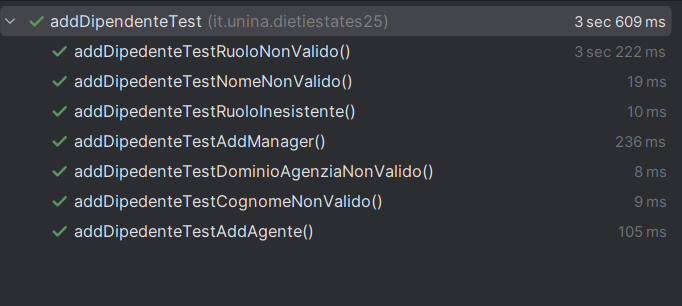
\includegraphics[width=0.7\linewidth]{Immagini/unit test/esitiTestAddDipendente.png}
	\caption[Esito test]{Screen che riporta l'esito positivo dei test}
\end{figure}
